\documentclass[a4paper,12pt,twoside]{book}

\usepackage{setspace}
\usepackage[T1]{fontenc}
\usepackage[utf8]{inputenc}
\usepackage{lmodern}
\usepackage[english,french]{babel}
\usepackage{geometry}
\usepackage{hyperref}
\usepackage{xcolor}
\usepackage{graphicx}
\usepackage{csquotes}
\usepackage{enumitem}
\usepackage{titlesec}
\usepackage{etoolbox}
\usepackage{fancyhdr,emptypage}
% fncychap retiré : titres compacts définis via titleformat ci-dessous
\usepackage{bookmark}
\usepackage[nottoc]{tocbibind}
\usepackage[
  backend=biber,
  style=apa,
  natbib=true,
  date=year,
  sorting=nyt,
  autolang=other,
]{biblatex}
\DeclareLanguageMapping{french}{french-apa}
\DeclareLanguageMapping{english}{english-apa}

\geometry{
  a4paper,
  left=3cm,
  right=2cm,
  top=3cm,
  bottom=3cm,
  headheight=28pt,
  marginparwidth=22mm
}

\raggedbottom
\reversemarginpar
\setcounter{tocdepth}{3}
\setcounter{secnumdepth}{3}
\addto\captionsfrench{\renewcommand{\chaptername}{Partie}}

\hypersetup{
  colorlinks=true,
  linkcolor={blue},
  filecolor={maroon},
  citecolor={blue},
  urlcolor={blue}
}

\fancypagestyle{plain}{
    \fancyhead{}
    \fancyfoot[C]{\thepage}
    \renewcommand{\headrulewidth}{0pt}
    \renewcommand{\footrulewidth}{0pt}
}

\pagestyle{fancy}
\fancyhf{}
\fancyhead[LE]{\selectfont\nouppercase{\leftmark}}
\fancyhead[RO]{\selectfont\nouppercase{\rightmark}}
\fancyfoot[C]{\thepage}

% --- Titres compacts (pas de page vide, tailles réduites) ---
\makeatletter
\patchcmd{\chapter}{\if@openright\cleardoublepage\else\clearpage\fi}{\par\vspace{1.5em}}{}{}
\patchcmd{\chapter}{\thispagestyle{plain}}{\thispagestyle{fancy}}{}{}
\makeatother

\titleformat{\chapter}[hang]
  {\normalfont\Large\bfseries}
  {\textcolor{blue}{Partie~\thechapter\enspace---\enspace}}{0pt}{}
\titlespacing*{\chapter}{0pt}{1.5em}{0.8em}

\titleformat{\section}
  {\normalfont\large\bfseries}{}{0pt}{}
\titlespacing*{\section}{0pt}{1em}{0.5em}

\titleformat{\subsection}
  {\normalfont\normalsize\bfseries}{}{0pt}{}
\titlespacing*{\subsection}{0pt}{0.8em}{0.4em}

\renewcommand{\baselinestretch}{1.2}

\addbibresource{bibliographie_air_interieur.bib}

\AtEveryCite{%
  \normalfont\normalcolor%
  \renewcommand*{\mkbibnamefamily}[1]{#1}%
  \renewcommand*{\mkbibnamegiven}[1]{#1}%
}

\title{Responsabiliser les ménages, invisibiliser les producteurs ?}
\makeatletter
\providecommand{\subtitle}[1]{%
  \apptocmd{\@title}{\par {\large #1 \par}}{}{}
}
\makeatother
\subtitle{La pollution de l'air intérieur comme problème public en France}
\author{Olivier CARON \and Emma GENTILE \and Tara L'HORTY \and Maryne NETO}
\date{15 avril 2026}

\begin{document}
\hypersetup{pageanchor=false}
\pagenumbering{gobble}
\begin{titlepage}
\thispagestyle{empty}
\begin{center}
{\Huge\bfseries Responsabiliser les ménages, invisibiliser les producteurs ?\par}
\vspace{0.35cm}
{\Large La pollution de l'air intérieur comme problème public en France\par}
\vspace{0.8cm}
{\large Sociologie de l'action publique\par}
\vspace{0.15cm}
{\normalsize Mineure Action Publique\par}
\vspace{0.8cm}
Olivier CARON \quad -- \quad Emma GENTILE \quad -- \quad Tara L'HORTY \quad -- \quad Maryne NETO\\
\vspace{0.5cm}
\textit{Les quatre auteurs ont contribué à parts égales à ce travail.}\\
\vspace{0.2cm}
15 avril 2026
\end{center}

\vspace{0.5cm}
\noindent\textbf{Résumé}\par
\smallskip
Cette note de recherche analyse la pollution de l'air intérieur comme problème public en France. Elle part d'un paradoxe : alors même que le risque sanitaire est aujourd'hui bien documenté par l'expertise, la quantification et l'action administrative, l'action publique privilégie surtout des instruments informationnels, comportementaux et procéduraux qui ciblent les occupants, plutôt que des dispositifs plus contraignants visant les producteurs, les bailleurs ou les professionnels du bâtiment. L'argument défendu est que cette configuration tient à la forme même de la publicisation du problème : visible, mais surtout dans des arènes expertes et dispersées ; objectivé, mais difficile à imputer politiquement de manière stable. Dans ce contexte, l'État gouverne moins par redistribution frontale des responsabilités que par étiquetage, recommandations de comportement, surveillance et vigilance continue. L'analyse montre enfin que cette faible conflictualité n'est pas socialement neutre : les prescriptions publiques supposent des ressources matérielles que les ménages les plus exposés possèdent le moins souvent.

\vfill
\begin{center}
    \begin{minipage}{.3\textwidth}
      \centering
      
\includegraphics[width=0.40\linewidth]{../devoir/assets/LOGO-PSL-nov-2017.png}
    \end{minipage}%
    \begin{minipage}{.3\textwidth}
      \centering
      
\includegraphics[width=.62\linewidth]{../devoir/assets/logo_ens_psl_en_png.png}
    \end{minipage}%
    \begin{minipage}{.3\textwidth}
      \centering
      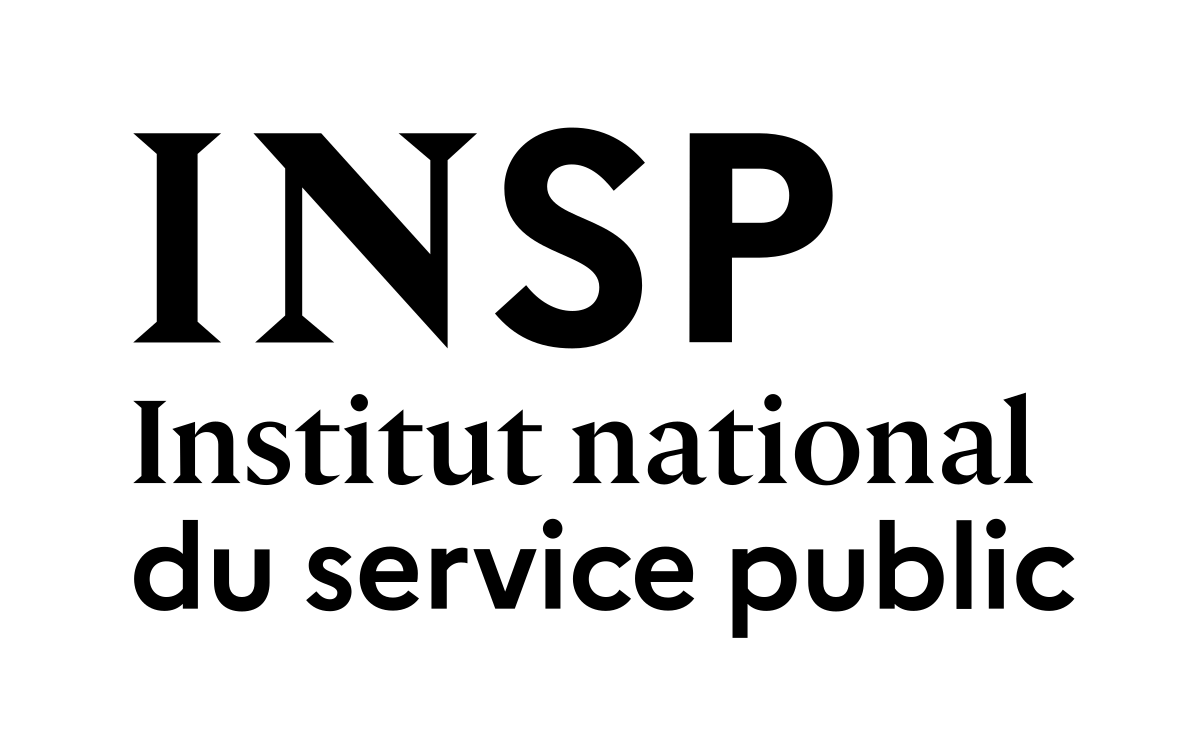
\includegraphics[width=.44\linewidth]{../devoir/assets/Logo_INSP.svg.png}
    \end{minipage}

    \vspace{0.3cm}

    Mineure Action Publique
\end{center}
\end{titlepage}

\newpage
\frontmatter
\renewcommand*{\contentsname}{Table des matières}
{
\hypersetup{linkcolor=}
\setcounter{tocdepth}{1}
\tableofcontents
}
\newpage
\mainmatter
\hypersetup{pageanchor=true}
\setstretch{1.25}

\chapter{Introduction}

La pollution de l'air intérieur est un problème sanitaire bien documenté. Elle reste pourtant un objet politique étonnamment discret. Depuis plus de vingt ans, l'Observatoire de la qualité de l'air intérieur, puis l'Observatoire de la qualité des environnements intérieurs, les plans nationaux santé-environnement, les avis de l'Anses et les publications du ministère de la Transition écologique accumulent mesures, estimations et recommandations qui établissent sans ambiguïté que l'air respiré dans les logements, les écoles ou les bureaux constitue un enjeu de santé publique \parencite{PlanQAI2013,MinistereEcologieQAI2025,OQAI2025CNL1,OQAI2025CNL2}. Cette montée en objectivation n'a pourtant pas débouché sur une politique fortement contraignante visant prioritairement les producteurs de matériaux, les bailleurs ou les professionnels du bâtiment. Elle a produit un ensemble d'instruments graduels, souvent peu conflictuels, qui informent, surveillent, orientent et responsabilisent.

Trois exemples suffisent à faire apparaître ce paradoxe. L'étiquetage des émissions de composés organiques volatils (COV) sur les produits de construction et de décoration vise bien les producteurs, mais par un instrument de classement et de transparence, non par une interdiction des produits les plus émissifs \parencite{Decret2011COV,Arrete2011COV,MinistereEcologieEtiquetageCOV2025}. La multiplication des guides de bonnes pratiques destinés aux ménages recommande d'aérer, de ventiler, de choisir les bons produits et d'entretenir les équipements \parencite{ADEME2024AirSainChezSoi,ADEME2023BienVentiler}. La surveillance de la qualité de l'air dans les établissements recevant du public s'organise autour de mesures de CO\textsubscript{2}, d'autodiagnostics et de plans d'action --- autour d'une logique de vigilance continue plus que de sanction \parencite{Decret2022ERP,HCSP2022CO2ERP}.

La question n'est donc pas d'abord sanitaire ; elle est sociologique. Il ne s'agit pas d'établir que le risque existe, mais d'expliquer pourquoi un problème pourtant objectivé donne lieu à cette forme d'action publique plutôt qu'à une autre. Les travaux sur la mise à l'agenda, la construction des problèmes publics, la quantification, le gouvernement des risques et l'instrumentation de l'action publique offrent ici un cadre opérant \parencite{Kingdon1984Agendas,ChailleuxZittoun2021GazSchiste,Ogien2010ValeurSocialeChiffre,Gusfield1981CulturePublicProblems,Borraz2008PolitiquesRisque,LascoumesLeGales2004GouvernerParLesInstruments}. Notre hypothèse est la suivante : la pollution de l'air intérieur devient bien un problème public, mais sa publicisation reste surtout experte, diffuse et faiblement conflictuelle ; cette configuration rend l'imputation des responsabilités politiquement coûteuse et favorise des instruments de faible conflictualité qui déplacent vers les occupants une part décisive de la gestion du risque. L'enjeu n'est pas d'affirmer qu'il s'agirait d'un problème \og sans responsable \fg, mais de montrer comment la responsabilité est diffusée, déplacée et politiquement amortie.

Le raisonnement procède en quatre temps : la publicisation experte et dispersée du risque ; les obstacles à une imputation politique stable ; les instruments de faible conflictualité qui déplacent la gestion vers les occupants ; enfin, les effets sociaux inégaux de cette configuration.

\section{Corpus et démarche}

Le corpus combine trois ensembles de matériaux. Le premier est constitué des travaux de sociologie de l'action publique qui forment le cadre théorique : mise à l'agenda, construction des problèmes publics, gouvernement des risques, instrumentation, mise en œuvre et changement \parencite{Kingdon1984Agendas,Gusfield1981CulturePublicProblems,Borraz2008PolitiquesRisque,GilbertHenry2012ProblemesPublics,LascoumesLeGales2004GouvernerParLesInstruments,HalpernLascoumesLeGales2014Instrumentation}. Le deuxième rassemble la littérature centrée sur l'air intérieur : travaux sur la faible scandabilité du problème, sur la tension entre régulation et responsabilisation, sur l'étiquetage, sur les pratiques domestiques et sur les dimensions matérielles du logement \parencite{LeBourhis2019AirInterieurResponsabilisation,CrespinFerron2016ScandaleRecherchePublic,HourcadeLeBourhis2024PolitiqueEtiquette,FerronLeBourhis2020DeconstruireProblemesPublics,MinoustchinVeraNavas2010RepresentationsComportementsQAI,Ginestet2020MouldIndoorEnvironments}. Le troisième réunit des sources institutionnelles et réglementaires : plans publics, rapports, décrets, guides, jurisprudences et tableaux de bord \parencite{PlanQAI2013,Decret2011COV,Decret2022ERP,Anses2016MoisissuresBati,FondationAbbePierre2013PrecariteSante,ONPE2024TableauBord}.

La démarche n'est ni une revue de littérature ni un inventaire d'instruments. Elle consiste à suivre un problème public à travers plusieurs opérations successives : son objectivation, sa circulation entre arènes, les obstacles à une imputation stable des responsabilités, puis la sélection d'instruments qui font porter l'ajustement sur certains acteurs plutôt que sur d'autres. Ce fil permet de croiser des matériaux hétérogènes sans les juxtaposer mécaniquement, et d'éviter deux impasses symétriques : traiter l'air intérieur comme une pure question technique, ou le réduire à l'énoncé normatif selon lequel l'État ne ferait pas assez.

\chapter{Publiciser un risque sans le transformer en scandale}

La pollution de l'air intérieur n'est ni un angle mort scientifique ni un impensé administratif. Depuis le début des années 2000, elle est mesurée, suivie, documentée et intégrée à plusieurs politiques publiques. Cette montée en visibilité ne prend pourtant pas la forme d'une grande politisation conflictuelle. Le problème devient public sans se transformer en scandale durable. Et c'est là que le problème se noue : un problème reconnu mais faiblement scandalisé a davantage de chances d'être traité par expertise, coordination et instruments graduels que par désignation d'un responsable central.

\section{Quantifier le problème pour le rendre gouvernable}

La première opération est une opération de mesure. Les campagnes nationales de l'OQAI, puis de l'OQEI, sortent l'exposition du registre de l'impression diffuse pour la stabiliser par des protocoles, des questionnaires et des séries comparables. La seconde campagne nationale, conduite entre la fin de 2020 et le début de 2023, porte sur 571 logements, répartis dans 321 communes et 84 départements \parencite{OQAI2025CNL1,OQAI2025CNL2}. Cette infrastructure ne produit pas seulement des données ; elle donne au problème une existence administrative, nationale et durable. Elle transforme des situations domestiques dispersées en objet gouvernable.

Le Plan QAI de 2013 prolonge ce travail de mise en forme. Il ne rappelle pas simplement qu'il existe des polluants ou des risques sanitaires ; il convertit l'air intérieur en domaine d'action publique doté de priorités, de publics cibles, de dispositifs et de responsabilités administratives \parencite{PlanQAI2013}. L'apport d'\textcite{Ogien2010ValeurSocialeChiffre} est ici direct : le chiffre ne décrit pas un problème préexistant ; il le rend calculable, comparable et administrable. Lu avec \textcite{Borraz2008PolitiquesRisque}, ce moment de quantification peut aussi se comprendre comme une dé-familiarisation. Des pratiques ordinaires --- chauffer, bricoler, meubler, ventiler, habiter --- cessent d'aller de soi lorsqu'elles deviennent lisibles à travers des concentrations, des seuils, des classes d'émission et des coûts sanitaires.

\section{Une visibilité dispersée, experte et peu politisée}

Cette objectivation ne passe pas par une arène unique. PNSE, pages ministérielles, interventions parlementaires, rapports du Sénat, travaux de l'OQAI/OQEI et avis d'expertise ne produisent pas la même visibilité, mais ils contribuent ensemble à stabiliser le sujet \parencite{PNSE32014Mesures,PNSE42022Rapport,MinistereEcologieQAI2025,QuestionAN2019OQAI,Senat2015CoutInaction}. Les travaux de \textcite{ChailleuxZittoun2021GazSchiste} sont utiles ici : ils permettent de penser la carrière d'un problème qui circule entre plusieurs espaces de débat sans trouver de propriétaire politique unique. L'air intérieur ne relève pas d'une inscription massive sur un agenda décisionnel central ; il relève d'une présence continue, mais fragmentée, dans plusieurs univers administratifs et experts.

Avec \textcite{Kingdon1984Agendas}, on peut dire que l'air intérieur accède bien à l'\emph{agenda gouvernemental} --- il circule dans les rapports, les plans et les arènes administratives --- sans nécessairement entrer dans l'\emph{agenda de décision}, là où des arbitrages plus coûteux seraient tranchés.

Cette dispersion est aussi médiatique. \textcite{CrespinFerron2016ScandaleRecherchePublic} montrent que l'air intérieur accède aux médias sous une forme faible, didactique et éclatée, loin du format du grand scandale sanitaire. Le rapport sénatorial de 2015 rappelle certes que l'OQAI a été créé en 2001 dans un contexte encore marqué par l'amiante, mais la trajectoire du sujet débouche sur une multiplication d'outils de coordination, de mesure et de recommandation \parencite{Senat2015CoutInaction}. La réponse gouvernementale à la question orale de 2019 sur l'avenir de l'observatoire confirme cette logique : elle met en avant des groupes de travail et des coordinations interministérielles, non une réforme conflictuelle \parencite{QuestionAN2019OQAI}.

La montée en visibilité est enfin portée par des milieux experts capables de stabiliser des méthodes, des indicateurs et un langage légitime du problème. L'OQAI, l'Anses, les services ministériels, les experts sanitaires et les producteurs de guides techniques ne fournissent pas seulement des connaissances ; ils contribuent à fixer la manière recevable de formuler le problème. \textcite{FerronHourcadeLeBourhis2022ApproprierProblemeAirInterieur} parlent à ce propos d'un cadrage refroidi : la construction du problème s'appuie sur un rapport structurellement inégal entre bureaucraties techniques, capables de stabiliser indicateurs, méthodes et vocabulaires, et un champ journalistique qui ne parvient pas à transformer le sujet en controverse durable.

Avec \textcite{GilbertHenry2012ProblemesPublics}, on peut qualifier plus précisément cette configuration. Le problème de l'air intérieur est bien \emph{publicisé} : il circule entre arènes, il est mesuré, documenté, administré. Il reste en revanche faiblement \emph{politisé}, au sens où les compromis qui structurent son traitement ne sont pas véritablement sortis des arènes spécialisées pour être rediscutés dans l'espace public général --- ce que \textcite{GilbertHenry2012ProblemesPublics} appellent le \emph{déconfinement} d'un problème. Les arbitrages entre santé, coût réglementaire, pratiques industrielles et viabilité sectorielle se stabilisent largement dans des espaces techniques et administratifs, sans être durablement reformulés dans le débat public général. C'est ce point qui ouvre la question suivante : comment un problème aussi objectivé peut-il rester aussi difficile à imputer ?

\chapter{L'objectivation sans imputation : pourquoi documenter un risque ne suffit pas à désigner un responsable}

Le fait que l'air intérieur soit mesuré, suivi et reconnu n'implique pas qu'il produise une désignation stable des responsables. Le c\oe ur du problème est là. L'objectivation scientifique existe, mais elle ne se convertit pas spontanément en attribution politique claire. Cette difficulté tient à la structure même de l'objet : risque invisible, absence d'événement focal, pluralité des sources, articulation instable entre causes, responsabilités juridiques et responsabilités politiques.

\section{Un risque réel, mais peu compatible avec la forme du scandale}

\textcite{LeBourhis2019AirInterieurResponsabilisation} a raison d'insister sur la position très particulière de l'air intérieur, situé à l'intersection du sanitaire, du logement, de la consommation et des pratiques domestiques. Un tel problème ne se laisse pas facilement dramatiser. \textcite{Bedeau2020InvisibleEnemy} parlent d'un \og ennemi invisible \fg : avant même de devenir conflictuel, le risque doit être rendu intelligible. Il faut l'équiper par des données, des dispositifs de mesure et un vocabulaire expert. Cette médiation technique ralentit déjà la possibilité d'une montée en crise.

Le problème ne bénéficie pas non plus des ressorts symboliques les plus efficaces de la mise en scandale. Ni catastrophe ponctuelle, ni auteur évident, ni groupe de victimes constitué autour d'un événement déclencheur. Comme le montrent \textcite{CrespinFerron2016ScandaleRecherchePublic}, la médiatisation reste informative et pédagogique, sans construire le moment de rupture qui transformerait l'affaire en controverse publique centrale. L'air intérieur est un problème documenté ; il n'est pas un problème politiquement dramatisé.

\section{Des causes nombreuses, une responsabilité politique instable}

La seconde difficulté vient de la structure causale. La pollution de l'air intérieur ne se ramène pas à une source unique. Moisissures, humidité, défaut de ventilation, composés organiques volatils issus des matériaux, pratiques de bricolage, usages domestiques et insuffisance de chauffage s'entrecroisent d'un logement à l'autre. Le rapport de l'Anses sur les moisissures dans le bâti insiste sur cette hétérogénéité tout en rappelant des effets sanitaires robustes ; il mentionne notamment des preuves fortes suggérant une causalité entre environnements humides et moisis et développement de l'asthme chez le jeune enfant \parencite{Anses2016MoisissuresBati}. \textcite{Ginestet2020MouldIndoorEnvironments} relient moisissures, ventilation, chauffage et précarité énergétique dans le cas français.

Le point important n'est pas qu'il n'y aurait pas de causes identifiables. Il est que leur pluralité rend la désignation d'un responsable principal techniquement contestable et politiquement coûteuse. \textcite{FerronLeBourhis2020DeconstruireProblemesPublics} invitent à dénaturaliser la catégorie d'\og air intérieur \fg : elle agrège sous une même dénomination administrative des situations, des espaces et des responsabilités très hétérogènes. Avec \textcite{Gusfield1981CulturePublicProblems}, on peut dire que le problème se heurte à un découplage persistant entre \emph{causal responsibility} et \emph{political responsibility}. Identifier des sources plausibles ne suffit pas à désigner l'institution ou l'acteur qui devrait publiquement \og faire quelque chose \fg. C'est cette dissociation qui empêche la fixation d'une chaîne d'imputation simple et durable.

\section{Du risque sanitaire au risque politique}

Le cas des bailleurs illustre cette difficulté. Les ressources de l'ANIL montrent que l'humidité, les moisissures, la condensation et les défauts de ventilation peuvent fonder des constats de non-décence ou d'insalubrité \parencite{ANILJurisprudence2025,ANILHabitatIndigne2025}. Mais cette voie juridique n'aboutit que rarement à une imputation collective stabilisée. Elle individualise la preuve, multiplie les expertises et laisse souvent place à des controverses sur le partage des responsabilités entre bailleur et locataire. Lu avec \textcite{Gusfield1981CulturePublicProblems}, ce contentieux montre qu'une responsabilité causale peut être établie au cas par cas sans produire pour autant une responsabilité politique générale.

C'est ici que \textcite{Borraz2008PolitiquesRisque} devient décisif. Le chapitre 5 montre que l'expertise scientifique ne réduit pas seulement l'incertitude sanitaire ; elle permet aussi aux pouvoirs publics de gérer le \emph{risque politique}. En réduisant et en convertissant certaines incertitudes, elle aide l'État à arbitrer entre protection sanitaire, coûts réglementaires et maintien de relations praticables avec des intérêts organisés. Plus largement, le rapport sénatorial de 2015 sur le coût de l'inaction en matière de pollution de l'air donne à voir ce type d'arbitrage : lors d'auditions de représentants de BASF France, de Bayer et de l'Union des industries chimiques, l'idée d'une réglementation trop spécifiquement française est explicitement associée au risque de distorsion, de délocalisation des outils de production et de perte de visibilité pour des cycles d'investissement longs \parencite{Senat2015CoutInaction}. L'imputation est donc difficile non seulement parce que la causalité est diffuse, mais parce qu'une mise en cause frontale redistribuerait immédiatement des coûts politiques et économiques.

La difficulté d'imputation ne bloque pas l'action publique ; elle l'oriente. Lorsqu'un problème sanitaire est objectivé mais reste coûteux à politiser, l'État a de fortes chances de privilégier des instruments qui organisent les conduites plutôt que de redistribuer frontalement les responsabilités. C'est exactement ce que montrent les instruments effectivement déployés sur l'air intérieur.

\chapter{Gouverner par l'information et la vigilance : des instruments qui déplacent la responsabilité vers les occupants}

L'air intérieur n'est pas un domaine d'inaction. Il est traité par une série d'instruments bien identifiables. La question est de savoir ce qu'ils font. Lu à partir de la typologie proposée par \textcite{lascoumesConclusionLinnovationInstrumentale2005}, le dossier combine surtout des instruments \emph{informatifs et communicationnels}, associés à l'explicitation des décisions et à la responsabilisation des acteurs, avec des \emph{normes et standards} à légitimité technico-scientifique et négociée. Ce choix n'est pas secondaire. Il dit comment l'État conçoit le problème et qui il considère comme premier opérateur de la réduction du risque.

\section{Étiqueter les produits plutôt qu'interdire les filières}

L'étiquetage des émissions de COV sur les produits de construction et de décoration fournit le cas le plus net. Le décret de 2011, son arrêté d'application et la présentation ministérielle montrent que les fabricants sont bien visés, mais principalement par une obligation d'information : à compter du 1\textsuperscript{er} septembre 2013, les produits doivent être classés de A+ à C selon leurs émissions, et la sanction porte d'abord sur l'absence d'étiquetage \parencite{Decret2011COV,Arrete2011COV,MinistereEcologieEtiquetageCOV2025}. Il s'agit d'un instrument de transparence obligatoire, non d'une interdiction des produits les plus émissifs.

Cette configuration nuance l'idée selon laquelle les producteurs seraient totalement hors champ. Ils sont régulés, mais selon une forme particulière de régulation. \textcite{Scutaru2020RiskMitigation} rappellent que les exigences contraignantes sur les émissions de produits restent rares en Europe : au moment de leur étude, seuls trois pays disposent d'exigences nationales de ce type. La France n'est pas dans l'inaction ; elle choisit une voie compatible avec l'harmonisation technique et la logique du marché. \textcite{Gallon2020EmissionsConstructionProcess} montrent que les matériaux et les processus constructifs contribuent en amont à l'exposition future des occupants. Pourtant, comme le soulignent \textcite{HourcadeLeBourhis2024PolitiqueEtiquette}, c'est l'étiquetage qui s'est imposé, non une politique plus frontale sur la qualité du bâti, les matériaux autorisés ou la responsabilité des propriétaires.

Ce déplacement se comprend avec \textcite{borrazChapitre3Normes2005}. Les normes et standards apparaissent comme des instruments politiquement efficaces parce qu'ils combinent rationalité scientifique et technique avec rationalité négociée, tout en conservant une apparence de neutralité. Ils permettent d'agir sans transformer immédiatement le problème en affrontement direct avec les secteurs concernés. Viser les producteurs par classement n'est pas équivalent à les contraindre par interdiction ; c'est déjà une manière spécifique de gouverner.

\section[Les occupants comme premiers gestionnaires de leur exposition]{Faire des occupants les premiers gestionnaires de leur exposition}

L'autre versant, plus massif, est la responsabilisation des ménages. Les guides de l'ADEME, le Plan QAI et une large part de la communication publique dessinent un occupant actif, informé, capable d'agir sur son environnement domestique. Aérer, ventiler, choisir des produits moins émissifs, entretenir les équipements, surveiller l'humidité, éviter certains usages : l'action publique passe ici par une pédagogie des gestes ordinaires \parencite{ADEME2024AirSainChezSoi,ADEME2023BienVentiler,PlanQAI2013}. C'est ce que \textcite{HourcadeLeBourhis2024PolitiqueEtiquette} montrent à propos de la \og politique de l'étiquette \fg : la régulation se déplace vers un consommateur supposé capable d'arbitrer ses choix et d'ajuster ses pratiques.

Cette logique ne va pas de soi. \textcite{MinoustchinVeraNavas2010RepresentationsComportementsQAI} montrent que les recommandations expertes rencontrent, dans les logements, des routines, des perceptions sensorielles, des contraintes matérielles et des rationalités pratiques irréductibles à la réception passive de l'information. L'instrument n'est jamais neutre. Avec \textcite{LascoumesLeGales2004GouvernerParLesInstruments}, on peut dire qu'il embarque une théorie du problème et de sa solution : si les guides sont centraux, c'est que l'action publique suppose qu'une part décisive de l'ajustement doit se jouer dans les conduites domestiques.

\section{Surveiller les ERP plutôt que sanctionner en amont}

Le cas des établissements recevant du public montre que l'action publique se structure plus aisément lorsque des publics sensibles, notamment les enfants, sont concernés. Mais même ici, la régulation prend d'abord une forme procédurale. Depuis le 1\textsuperscript{er} janvier 2023, la surveillance de la qualité de l'air intérieur dans certains établissements repose sur une évaluation annuelle des moyens d'aération avec mesure du CO\textsubscript{2}, un autodiagnostic tous les quatre ans et un plan d'action \parencite{Decret2022ERP,MinistereEcologieQAI2025}. L'avis du HCSP de 2022 complète ce cadrage en retenant une valeur repère à 800 ppm et une valeur d'action rapide à 1 500 ppm \parencite{HCSP2022CO2ERP}.

La présence d'enfants dans ces établissements rend l'intervention publique plus légitime : le risque est ici rapporté à un public dont la vulnérabilité fait consensus, ce qui réduit le coût politique de l'action. Pour autant, les conséquences d'un autodiagnostic défavorable restent largement internes au dispositif : elles déclenchent un plan d'action, non une fermeture ou une sanction directe. Même dans le cas le plus favorable à la régulation, l'État privilégie donc l'ajustement progressif à la mise en cause frontale.

Le problème est traité par des seuils, des capteurs, des procédures, des corrections graduelles. Il ne s'agit pas d'une absence de régulation, mais d'un gouvernement technique et continu qui organise la vigilance plus qu'il ne met en scène la sanction. Avec \textcite{palierChapitre7Instruments2005} et la conclusion de \textcite{lascoumesConclusionLinnovationInstrumentale2005}, on peut lire cette configuration comme un empilement d'instruments qui s'ajoutent, se recomposent et se spécialisent sans rupture d'ensemble. Même lorsqu'elle devient plus explicite, l'action publique sur l'air intérieur conserve une propriété centrale : elle agit en réglant les conduites, les routines de surveillance et les pratiques de gestion des espaces.

\chapter{Une politique qui individualise sans redistribuer}

La faible conflictualité de l'action publique ne dilue pas seulement les responsabilités. Elle produit aussi des effets sociaux inégaux. Les instruments dominants --- guides, autodiagnostics, étiquetage, surveillance procédurale --- paraissent universels. Ils présupposent en réalité des ressources matérielles, cognitives et organisationnelles très inégalement distribuées.

\section[Des prescriptions universelles en apparence]{Des prescriptions apparemment universelles, mais socialement sélectives}

Aérer quotidiennement, bien ventiler, chauffer correctement, entretenir les équipements, choisir les produits les moins émissifs : ces recommandations ne sont plausibles que si le logement le permet. Les guides de l'ADEME présupposent des fenêtres ouvrables, des systèmes de ventilation fonctionnels, un budget énergétique soutenable, des marges de choix sur les produits consommés et une capacité concrète à intervenir sur son environnement \parencite{ADEME2024AirSainChezSoi,ADEME2023BienVentiler}. La responsabilisation comportementale n'est jamais purement cognitive ; elle repose sur des conditions matérielles.

Le rapport Fondation Abbé Pierre / CREAI-ORS rend ce décalage particulièrement visible. L'enquête porte sur 362 logements et 750 personnes. Dans les ménages exposés à la précarité énergétique, 64,0 \% des logements présentent des moisissures contre 17,0 \% dans les autres ; 45,8 \% connaissent des infiltrations d'eau contre 13,5 \% ; et 26,2 \% ont des bouches d'aération bouchées contre 11,3 \% \parencite{FondationAbbePierre2013PrecariteSante}. Le tableau de bord 2024 de l'ONPE cadre cette tension à l'échelle macro : 79 \% des Français déclarent avoir réduit le chauffage pour limiter leurs factures et 26 \% disent avoir souffert du froid chez eux pendant l'hiver 2022-2023 \parencite{ONPE2024TableauBord}. Ces données portent sur la précarité énergétique, non directement sur la qualité de l'air intérieur ; mais le lien est direct : un ménage qui réduit le chauffage ou qui n'ouvre pas les fenêtres pour ne pas perdre de chaleur dégrade aussi, en pratique, sa ventilation et son exposition aux polluants intérieurs. Ces chiffres ne servent pas de décor. Ils montrent que les ménages sommés d'agir sur leur exposition sont aussi ceux qui disposent le moins des conditions matérielles pour suivre les prescriptions publiques.

\section{Un gouvernement des risques qui individualise sans redistribuer}

Le cas de l'air intérieur éclaire une forme plus générale d'action publique. Le problème est objectivé, équipé, suivi et outillé, mais son traitement repose largement sur des prescriptions individualisées et des ajustements locaux. \textcite{MontouroyBiabianyMassardier2022Declimatisation} aident à saisir ce déplacement : la mise en œuvre des instruments peut dépolitiser un problème en le rabattant sur des usages, des réglages et des comportements. Dans le cas de l'air intérieur, ce rabattement ne supprime pas le problème ; il en redéfinit le centre de gravité. Ce qui était aussi une question de production, de qualité du bâti, de ventilation structurelle et de politique du logement devient, en grande partie, une question de vigilance domestique et de capacité d'ajustement individuelle.

Ce déplacement s'inscrit dans une dynamique de sédimentation instrumentale. \textcite{palierChapitre7Instruments2005} permettent de nommer le phénomène : le changement passe moins par une rupture que par l'ajout de couches successives. La conclusion de \textcite{lascoumesConclusionLinnovationInstrumentale2005} précise les formes de ce processus : \og glissements \fg, \og reconversions-adaptations \fg et \og recyclages \fg plutôt qu'innovation radicale. La politique de l'air intérieur ne redistribue pas frontalement les responsabilités ; elle les redéploie par empilement d'instruments qui organisent progressivement qui doit surveiller, arbitrer, entretenir et corriger.

\chapter{Conclusion}

L'analyse permet de répondre nettement à la question de départ. Si l'action publique française privilégie des instruments informationnels, comportementaux et procéduraux en matière d'air intérieur, ce n'est ni parce que le problème serait mal connu, ni parce que l'État serait absent. C'est parce que la configuration même du problème favorise ce type de traitement. La pollution de l'air intérieur est publicisée et objectivée, mais sous une forme experte, dispersée et faiblement scandalisée. L'imputation politique des responsabilités reste difficile : les sources sont nombreuses, les chaînes causales hétérogènes, le droit individualise la preuve, et toute mise en cause frontale redistribuerait immédiatement des coûts économiques et politiques.

Le choix des instruments apparaît alors sous un autre jour. L'étiquetage, les guides, la surveillance dans les ERP et les dispositifs d'autodiagnostic ne sont pas des solutions purement techniques. Ce sont des choix politiques sur la forme acceptable de la régulation. Ils permettent d'agir sur le problème tout en limitant la conflictualité de cette action. Mais cette faible conflictualité a un prix. En faisant des occupants les premiers gestionnaires de leur exposition, l'action publique suppose des marges d'action qui sont précisément les moins disponibles dans les logements les plus dégradés, les plus humides, les moins bien ventilés et les plus exposés à la précarité énergétique.

La pollution de l'air intérieur n'apparaît donc pas comme un problème sans responsable. Elle apparaît comme un problème dont la responsabilité est diffusée, déplacée et politiquement amortie. Le cas de l'air intérieur rend visible une logique plus large : lorsque l'imputation est coûteuse et que les arbitrages restent confinés dans des espaces experts, l'État gouverne volontiers par l'information, la vigilance et l'ajustement des conduites avant de gouverner par la contrainte directe.

\chapter*{Note sur les usages de l'IA}
\addcontentsline{toc}{chapter}{Note sur les usages de l'IA}

La préparation de cette version de travail a mobilisé plusieurs outils d'intelligence artificielle. Ils ont servi au repérage bibliographique, à l'extraction de métadonnées, au classement de sources et à la constitution d'un corpus de travail à partir de Zotero, de PDF locaux et de ressources institutionnelles. Ils ont également permis de produire des synthèses intermédiaires, de tester la cohérence du plan, d'identifier des tensions entre références et de proposer des reformulations.

Plus concrètement, des outils conversationnels et de recherche assistée (\emph{Codex}, \emph{Claude Opus} et des connecteurs associés à Zotero) ont été utilisés pour repérer des références, extraire des résumés de travail, comparer des textes entre eux, tester plusieurs formulations de problématique et vérifier la cohérence d'ensemble du plan. Leur usage a été strictement encadré. Les références mobilisées dans le corps de la note ont été relues en plein texte avant d'être citées comme appuis substantiels. Les chiffres ont été revérifiés à partir des rapports et documents sources. Les reformulations proposées par ces outils n'ont été conservées qu'après réécriture et validation humaines. Les principaux avantages tiennent au gain de temps sur la cartographie du corpus, la mise en relation des textes et le contrôle de cohérence du raisonnement. Leurs limites sont apparues tout aussi nettement : risque de sur-généralisation, formulations trop lisses, confusion possible entre textes proches, tendance à gommer les hésitations ou les conflits qui font l'intérêt d'une enquête en sociologie de l'action publique. Les outils d'IA ont donc été utilisés comme instruments de préparation, de vérification et de reformulation ponctuelle, non comme substituts à la lecture des textes ni à la discussion collective des arguments.


\backmatter

\nocite{
Kingdon1984Agendas,
ChailleuxZittoun2021GazSchiste,
Hassenteufel2021SociologiePolitiqueActionPublique,
Ogien2010ValeurSocialeChiffre,
Matyjasik2014SourcesEvaluation,
Borraz2008PolitiquesRisque,
Gusfield1981CulturePublicProblems,
GilbertHenry2012ProblemesPublics,
LascoumesLeGales2004GouvernerParLesInstruments,
HalpernLascoumesLeGales2014Instrumentation,
Lamb2022Linky,
MontouroyBiabianyMassardier2022Declimatisation,
Palier2005InstrumentsTraceurs,
Sine2006IncrementalismeBudgetaire,
PressmanWildavsky1973Implementation,
Selznick1949TVA,
CrozierFriedberg1977ActeurSysteme,
LeBourhis2019AirInterieurResponsabilisation,
Bedeau2020InvisibleEnemy,
Ginestet2020MouldIndoorEnvironments,
Scutaru2020RiskMitigation,
Gallon2020EmissionsConstructionProcess,
Pal2024ExposureVOCs,
PlanQAI2013,
MinistereEcologieQAI2025,
PNSE32014Mesures,
PNSE42022Rapport,
Decret2011COV,
Arrete2011COV,
MinistereEcologieEtiquetageCOV2025,
Decret2022ERP,
HCSP2022CO2ERP,
OQAI2025CNL1,
OQAI2025CNL2,
QuestionAN2019OQAI,
Senat2015CoutInaction,
Anses2016MoisissuresBati,
FondationAbbePierre2013PrecariteSante,
ONPE2024TableauBord,
ANILJurisprudence2025,
ANILHabitatIndigne2025,
}

\nocite{ADEME2024AirSainChezSoi}
\nocite{ADEME2023BienVentiler}
\nocite{MinoustchinVeraNavas2010RepresentationsComportementsQAI}
\nocite{CrespinFerron2016ScandaleRecherchePublic}
\nocite{HourcadeLeBourhis2024PolitiqueEtiquette}
\nocite{FerronLeBourhis2020DeconstruireProblemesPublics}
\nocite{FerronHourcadeLeBourhis2022ApproprierProblemeAirInterieur}
\nocite{borrazChapitre3Normes2005}
\nocite{lascoumesConclusionLinnovationInstrumentale2005}
\nocite{palierChapitre7Instruments2005}

\begin{singlespace}
\small\printbibliography[heading=bibintoc,title=Bibliographie]
\end{singlespace}

\end{document}
